\documentclass[11pt,preprint, authoryear]{elsarticle}

\usepackage{lmodern}
%%%% My spacing
\usepackage{setspace}
\setstretch{1.2}
\DeclareMathSizes{12}{14}{10}{10}

% Wrap around which gives all figures included the [H] command, or places it "here". This can be tedious to code in Rmarkdown.
\usepackage{float}
\let\origfigure\figure
\let\endorigfigure\endfigure
\renewenvironment{figure}[1][2] {
    \expandafter\origfigure\expandafter[H]
} {
    \endorigfigure
}

\let\origtable\table
\let\endorigtable\endtable
\renewenvironment{table}[1][2] {
    \expandafter\origtable\expandafter[H]
} {
    \endorigtable
}


\usepackage{ifxetex,ifluatex}
\usepackage{fixltx2e} % provides \textsubscript
\ifnum 0\ifxetex 1\fi\ifluatex 1\fi=0 % if pdftex
  \usepackage[T1]{fontenc}
  \usepackage[utf8]{inputenc}
\else % if luatex or xelatex
  \ifxetex
    \usepackage{mathspec}
    \usepackage{xltxtra,xunicode}
  \else
    \usepackage{fontspec}
  \fi
  \defaultfontfeatures{Mapping=tex-text,Scale=MatchLowercase}
  \newcommand{\euro}{€}
\fi

\usepackage{amssymb, amsmath, amsthm, amsfonts}

\def\bibsection{\section*{References}} %%% Make "References" appear before bibliography


\usepackage[round]{natbib}

\usepackage{longtable}
\usepackage[margin=2.3cm,bottom=2cm,top=2.5cm, includefoot]{geometry}
\usepackage{fancyhdr}
\usepackage[bottom, hang, flushmargin]{footmisc}
\usepackage{graphicx}
\numberwithin{equation}{section}
\numberwithin{figure}{section}
\numberwithin{table}{section}
\setlength{\parindent}{0cm}
\setlength{\parskip}{1.3ex plus 0.5ex minus 0.3ex}
\usepackage{textcomp}
\renewcommand{\headrulewidth}{0.2pt}
\renewcommand{\footrulewidth}{0.3pt}

\usepackage{array}
\newcolumntype{x}[1]{>{\centering\arraybackslash\hspace{0pt}}p{#1}}

%%%%  Remove the "preprint submitted to" part. Don't worry about this either, it just looks better without it:
\makeatletter
\def\ps@pprintTitle{%
  \let\@oddhead\@empty
  \let\@evenhead\@empty
  \let\@oddfoot\@empty
  \let\@evenfoot\@oddfoot
}
\makeatother

 \def\tightlist{} % This allows for subbullets!

\usepackage{hyperref}
\hypersetup{breaklinks=true,
            bookmarks=true,
            colorlinks=true,
            citecolor=blue,
            urlcolor=blue,
            linkcolor=blue,
            pdfborder={0 0 0}}


% The following packages allow huxtable to work:
\usepackage{siunitx}
\usepackage{multirow}
\usepackage{hhline}
\usepackage{calc}
\usepackage{tabularx}
\usepackage{booktabs}
\usepackage{caption}


\newenvironment{columns}[1][]{}{}

\newenvironment{column}[1]{\begin{minipage}{#1}\ignorespaces}{%
\end{minipage}
\ifhmode\unskip\fi
\aftergroup\useignorespacesandallpars}

\def\useignorespacesandallpars#1\ignorespaces\fi{%
#1\fi\ignorespacesandallpars}

\makeatletter
\def\ignorespacesandallpars{%
  \@ifnextchar\par
    {\expandafter\ignorespacesandallpars\@gobble}%
    {}%
}
\makeatother

\newlength{\cslhangindent}
\setlength{\cslhangindent}{1.5em}
\newenvironment{CSLReferences}%
  {\setlength{\parindent}{0pt}%
  \everypar{\setlength{\hangindent}{\cslhangindent}}\ignorespaces}%
  {\par}


\urlstyle{same}  % don't use monospace font for urls
\setlength{\parindent}{0pt}
\setlength{\parskip}{6pt plus 2pt minus 1pt}
\setlength{\emergencystretch}{3em}  % prevent overfull lines
\setcounter{secnumdepth}{5}

%%% Use protect on footnotes to avoid problems with footnotes in titles
\let\rmarkdownfootnote\footnote%
\def\footnote{\protect\rmarkdownfootnote}
\IfFileExists{upquote.sty}{\usepackage{upquote}}{}

%%% Include extra packages specified by user

%%% Hard setting column skips for reports - this ensures greater consistency and control over the length settings in the document.
%% page layout
%% paragraphs
\setlength{\baselineskip}{12pt plus 0pt minus 0pt}
\setlength{\parskip}{12pt plus 0pt minus 0pt}
\setlength{\parindent}{0pt plus 0pt minus 0pt}
%% floats
\setlength{\floatsep}{12pt plus 0 pt minus 0pt}
\setlength{\textfloatsep}{20pt plus 0pt minus 0pt}
\setlength{\intextsep}{14pt plus 0pt minus 0pt}
\setlength{\dbltextfloatsep}{20pt plus 0pt minus 0pt}
\setlength{\dblfloatsep}{14pt plus 0pt minus 0pt}
%% maths
\setlength{\abovedisplayskip}{12pt plus 0pt minus 0pt}
\setlength{\belowdisplayskip}{12pt plus 0pt minus 0pt}
%% lists
\setlength{\topsep}{10pt plus 0pt minus 0pt}
\setlength{\partopsep}{3pt plus 0pt minus 0pt}
\setlength{\itemsep}{5pt plus 0pt minus 0pt}
\setlength{\labelsep}{8mm plus 0mm minus 0mm}
\setlength{\parsep}{\the\parskip}
\setlength{\listparindent}{\the\parindent}
%% verbatim
\setlength{\fboxsep}{5pt plus 0pt minus 0pt}



\begin{document}



\begin{frontmatter}  %

\title{Question 5}

% Set to FALSE if wanting to remove title (for submission)




\author[Add1]{Sahil Bhugwan}
\ead{21075492@sun.ac.za}







\begin{abstract}
\small{
Appalling Designs pitch for a new app based on past experaince
}
\end{abstract}

\vspace{1cm}





\vspace{0.5cm}

\end{frontmatter}



%________________________
% Header and Footers
%%%%%%%%%%%%%%%%%%%%%%%%%%%%%%%%%
\pagestyle{fancy}
\chead{}
\rhead{}
\lfoot{}
\rfoot{}
\lhead{}
%\rfoot{\footnotesize Page \thepage } % "e.g. Page 2"
\cfoot{}

%\setlength\headheight{30pt}
%%%%%%%%%%%%%%%%%%%%%%%%%%%%%%%%%
%________________________

\headsep 35pt % So that header does not go over title




\hypertarget{introduction}{%
\section{\texorpdfstring{Introduction
\label{Introduction}}{Introduction }}\label{introduction}}

Using Google play and user reports to compile an analysis on there being
new app for AppallingDesigns

\hypertarget{apps}{%
\section*{APPs}\label{apps}}
\addcontentsline{toc}{section}{APPs}

For the apps i will be looking at a few points

\begin{figure}[H]

{\centering \includegraphics{Q5_files/figure-latex/Figure1-1} 

}

\caption{APP ratings  \label{Figure1}}\label{fig:Figure1}
\end{figure}

It can bee seen that apps that have a rating between 4-5 tend to have
more downloads. It is also important to take note of for who the apps
are for.

\begin{figure}[H]

{\centering \includegraphics{Q5_files/figure-latex/Figure2-1} 

}

\caption{CONTENT   \label{Figure2}}\label{fig:Figure2}
\end{figure}

There is apps are for any age groups they tend to be most downloaded
this is because you have a wider audience.

\hypertarget{app-ratings}{%
\subsection{App ratings}\label{app-ratings}}

Important considerations to look at is that apps must be contentiously
updated as users want the new and best features all the time.

\begin{figure}[H]

{\centering 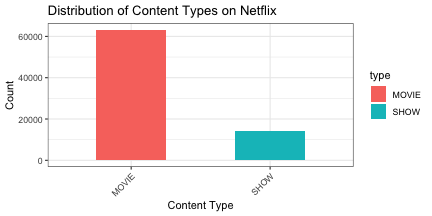
\includegraphics{Q5_files/figure-latex/Figure3-1} 

}

\caption{Ratings to update   \label{Figure3}}\label{fig:Figure3}
\end{figure}

therefore we can see that apps that have recently been update always
tend to be downloaded. However having to update your app will also
impact your clients memory on their phone.

\begin{figure}[H]

{\centering \includegraphics{Q5_files/figure-latex/Figure4-1} 

}

\caption{Rating to Size   \label{Figure4}}\label{fig:Figure4}
\end{figure}

Therefore apps need to be optimized so that they aren't to large for the
users .

\hypertarget{user-feedback}{%
\section{User Feedback}\label{user-feedback}}

It is vital that we get feedback from the user to ensure that we are
meeting there demands in an ever changing world.

\begin{figure}[H]

{\centering \includegraphics{Q5_files/figure-latex/Figure5-1} 

}

\caption{User Reviews  \label{Figure5}}\label{fig:Figure5}
\end{figure}

As we can see that the most common response is that users tend not to
answer this question. It would be vital to ensure that we get feedback
from them.

\begin{figure}[H]

{\centering \includegraphics{Q5_files/figure-latex/Figure6-1} 

}

\caption{App Sentiment   \label{Figure6}}\label{fig:Figure6}
\end{figure}

Looking at some of the apps it is important to ensure that users have a
great opion of the app as the app can be spread through good word of
mouth.

\hypertarget{conclusion}{%
\section{Conclusion}\label{conclusion}}

Therefore for Appalling Designs to design an app it must ensure that the
app is for everyone that way it can have a bigger reach. That is
regularly updated to keeps up with the changing demand, this will ensure
that user will have a great sentiment towards the app.

\bibliography{Tex/ref}





\end{document}
